\documentclass[10pt]{beamer}
\usetheme{Malmoe}
\colorlet{beamer@blendedblue}{green!40!black}
\setbeamertemplate{navigation symbols}{}
\newcommand*\oldmacro{}%
\let\oldmacro\insertshorttitle%
\renewcommand*\insertshorttitle{%
\oldmacro\hfill%
\insertframenumber\,/\,\inserttotalframenumber}

\usepackage{xfrac}
\usepackage{caption}
\usepackage{hyperref}
\usepackage[makeroom]{cancel}
\usepackage{ amssymb }
\usepackage{appendixnumberbeamer}
%\usepackage{tikz-feynman}
\usepackage{graphicx}
\begin{document}
\title{Search for Flavor Changing Neutral Currents in Top Quark Decays}
\subtitle{$t \rightarrow q \gamma$}
\subtitle{Fake Rates and Initial Asimov Fits}
\author[Barkeloo]{Jason Barkeloo}

\titlegraphic{
\includegraphics[width=4cm]{../ATLAS-Logo-Ref-RGB.png}\hspace*{2.75cm}~%
   
\includegraphics[width=4cm]{../uo_logo_green_on_white_2.jpg}
}

%\frame{\frametitle{}
%\begin{itemize}
%\item
%\end{itemize}
%}


\date{January 16, 2020}
\frame{\titlepage}
\frame{\frametitle{Overview}\tableofcontents[]}%hidesubsections]}
\section{Brief Background}
%\frame{\frametitle{Table of Contents}\tableofcontents[currentsection,hideothersubsections]}
%%%%%%%%%%%%%%%%%%%%%%%%%%%%%%%%%%%%%%%%%%%%%%%%%%%%%%%%%

\subsection{The Top Quark}

\frame{\frametitle{Top Quark Decays in the SM}
\centering
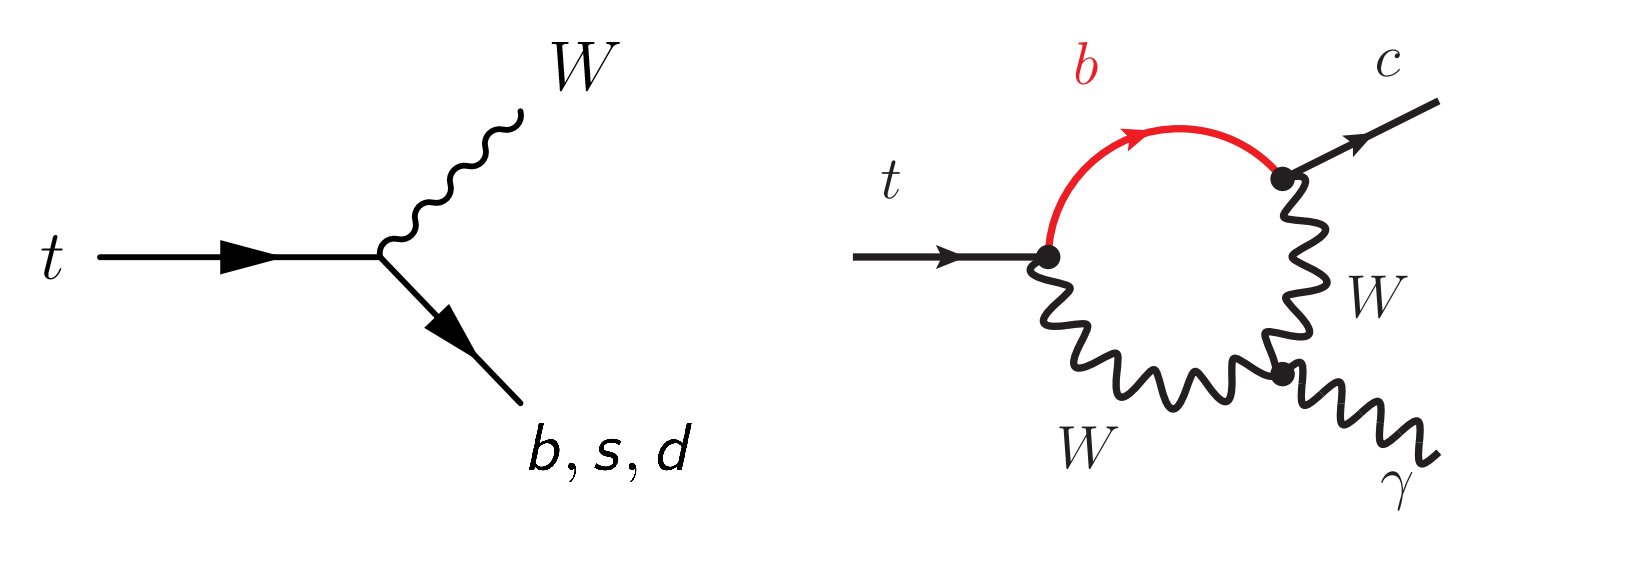
\includegraphics[width=1.\textwidth]{../../Thesis/ThesisImages/Theory/SMTopDecays2.png}

\begin{columns}
\begin{column}{0.5\textwidth}
\begin{itemize}
\item $t\rightarrow b W \approx 99.83\%$
\item $t\rightarrow s W \approx 0.16\%$
\item $t\rightarrow d W \approx 0.01\%$
\end{itemize}
\end{column}
\begin{column}{0.5\textwidth}
\begin{itemize}
\item $t\rightarrow q_{u,c} X\approx 10^{-17} - 10^{-12}$
\item Limits on $t\rightarrow \gamma q$ processes: \href{http://inspirehep.net/record/1750600?ln=en}{[Phys.Lett. B800 135082]}
	\begin{itemize}
	\item $t\rightarrow \gamma u < 2.8 x10^{-5}$
	\item $t\rightarrow \gamma c <  18 x 10^{-5}$
	\end{itemize}
\end{itemize}
\end{column}
\end{columns}
}



\subsection{FCNC at the LHC} 

\frame{\frametitle{FCNC: What are we looking for? $t\bar{t}\rightarrow W (\rightarrow l \nu) b+ q\gamma$}
Will further investigate BJets here.
\begin{itemize}
\item Final state topology
	\begin{itemize}
	\item One Neutrino, from W
	\item One Lepton, from W
	\item One B-jet, SM Top
	\item One Photon, FCNC Top
	\item One Jet, FCNC Top
	\end{itemize}
\end{itemize}
\centering
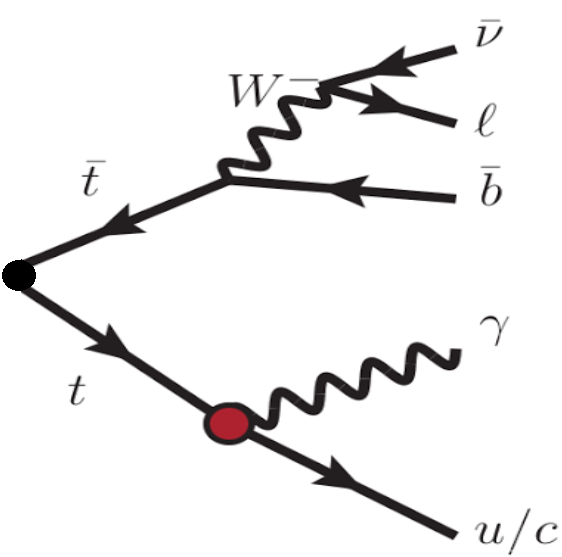
\includegraphics[width=0.35\textwidth]{../../Thesis/ThesisImages/fcncttbar.png}
}

\frame{\frametitle{Preselection NN Outputs}
\begin{columns}
\begin{column}{0.48\textwidth}
\begin{itemize}
\item $e$+jets
\end{itemize}
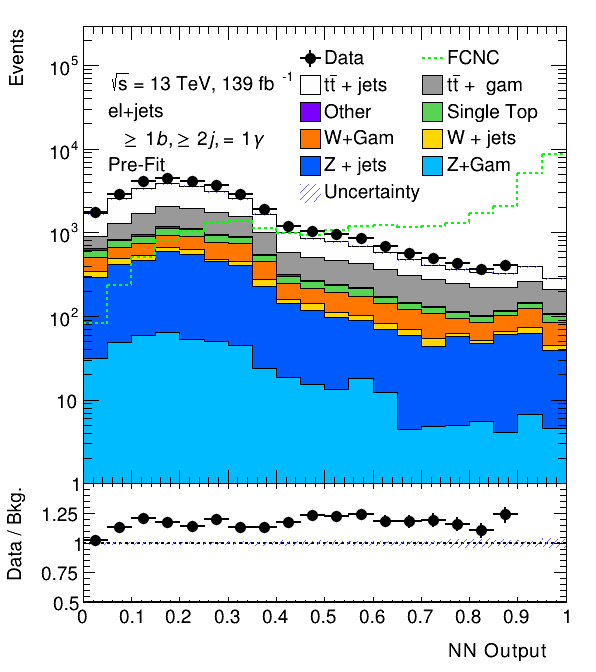
\includegraphics[width=.95\textwidth]{Images/PreSel_NNejet.png}
\end{column}
\begin{column}{0.48\textwidth}
\begin{itemize}
\item $\mu$+jets
\end{itemize}
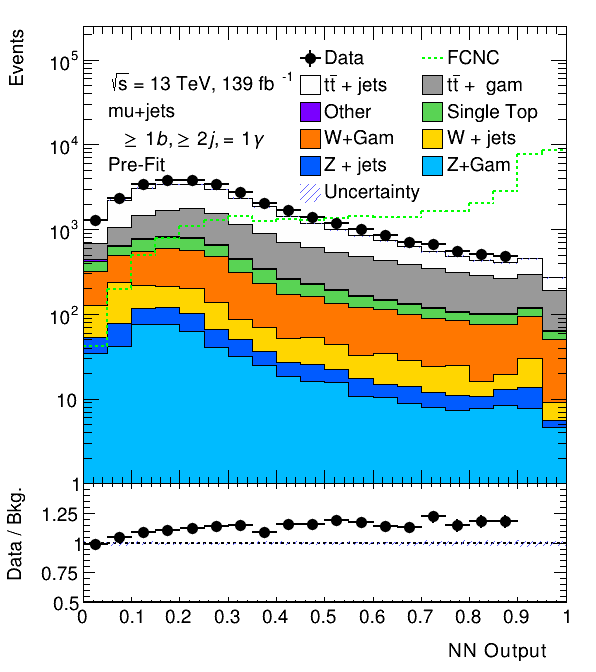
\includegraphics[width=.95\textwidth]{Images/PreSel_NNmujet.png}
\end{column}
\end{columns}
}
\subsection{Scale Factors for Non-Prompt Photon Samples}
\frame{\frametitle{No Photon Scale Factors}
\begin{columns}
\begin{column}{0.02\textwidth}
\rotatebox{90}{SF Applied \qquad Before SF\qquad} 
%\rotatebox{90}{Muon Channel        } 
\end{column}
\begin{column}{0.32\textwidth}
\begin{itemize}
\item W+jets Rich
\end{itemize}
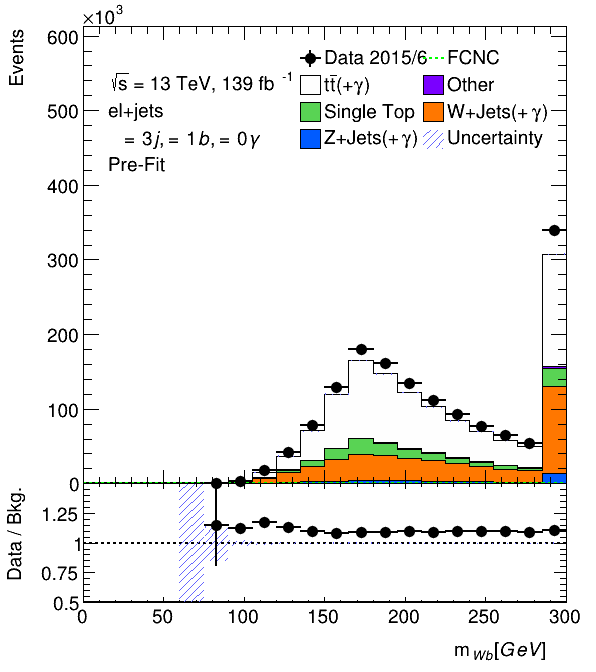
\includegraphics[width=.8\textwidth]{../../Thesis/ThesisImages/RegionPlots/AfterScaling/ControlRegions/HardCodedNormFactor/FCNC_All_ejets/Plots/CR1_SMtop.png} \\
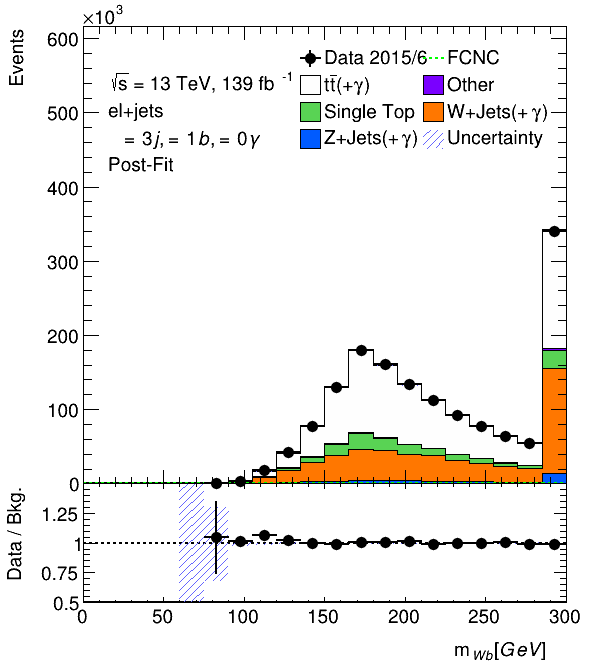
\includegraphics[width=.8\textwidth]{../../Thesis/ThesisImages/RegionPlots/AfterScaling/ControlRegions/HardCodedNormFactor/FCNC_All_ejets/Plots/CR1_SMtop_postFit.png} \\
\end{column}
\begin{column}{0.32\textwidth}
\begin{itemize}
\item $t\bar{t}$+jets Rich
\end{itemize}
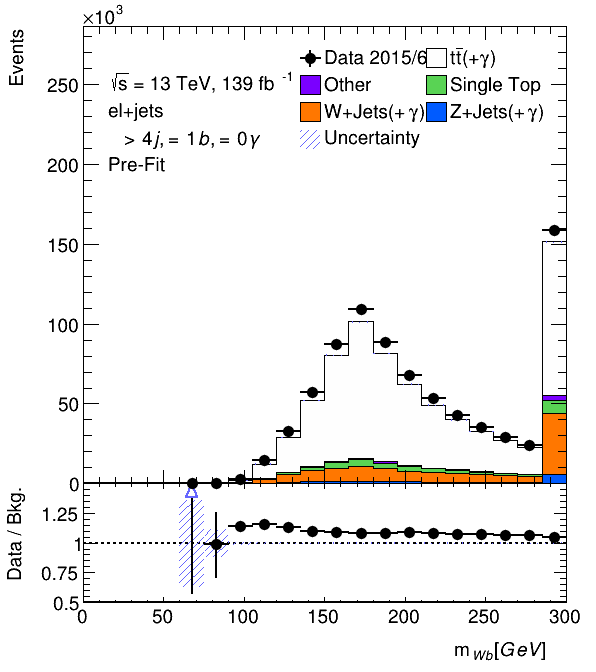
\includegraphics[width=.8\textwidth]{../../Thesis/ThesisImages/RegionPlots/AfterScaling/ControlRegions/HardCodedNormFactor/FCNC_All_ejets/Plots/CR2_SMtop.png} \\
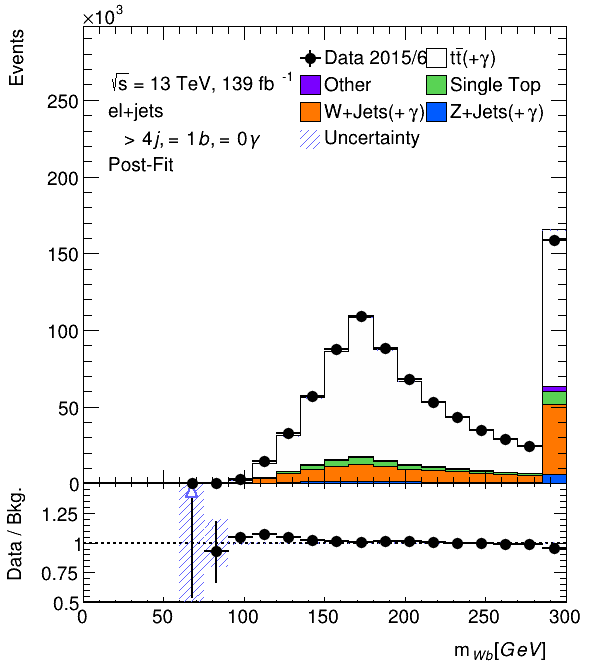
\includegraphics[width=.8\textwidth]{../../Thesis/ThesisImages/RegionPlots/AfterScaling/ControlRegions/HardCodedNormFactor/FCNC_All_ejets/Plots/CR2_SMtop_postFit.png}
\end{column}
\begin{column}{0.32\textwidth}
\begin{itemize}
\item Validation Region
\end{itemize}
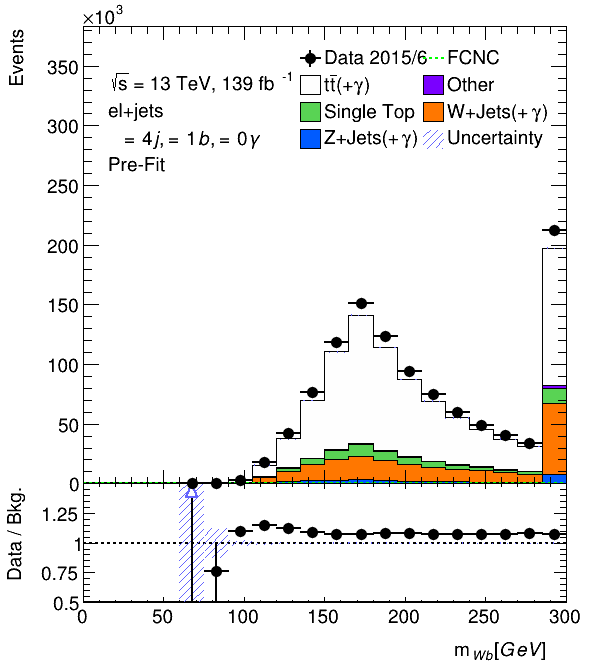
\includegraphics[width=.8\textwidth]{../../Thesis/ThesisImages/RegionPlots/AfterScaling/ControlRegions/HardCodedNormFactor/FCNC_All_ejets/Plots/VR3_SMtop.png} \\
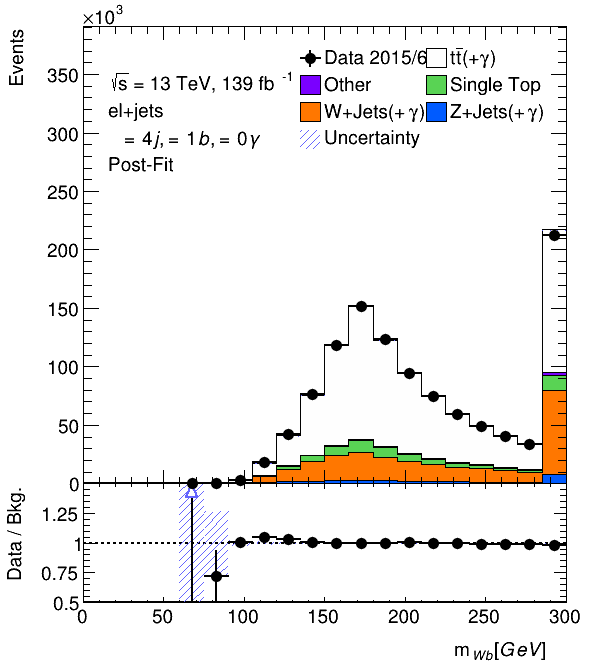
\includegraphics[width=.8\textwidth]{../../Thesis/ThesisImages/RegionPlots/AfterScaling/ControlRegions/HardCodedNormFactor/FCNC_All_ejets/Plots/VR3_SMtop_postFit.png}
\end{column}
\end{columns}
}

%%%%%%%%%%%%%%%%
\section{Fake Rate Studies}
\subsection{$e\rightarrow \gamma$ Fake Rate Studies}

\frame{\frametitle{Fake Rate Studies}
\begin{centering}
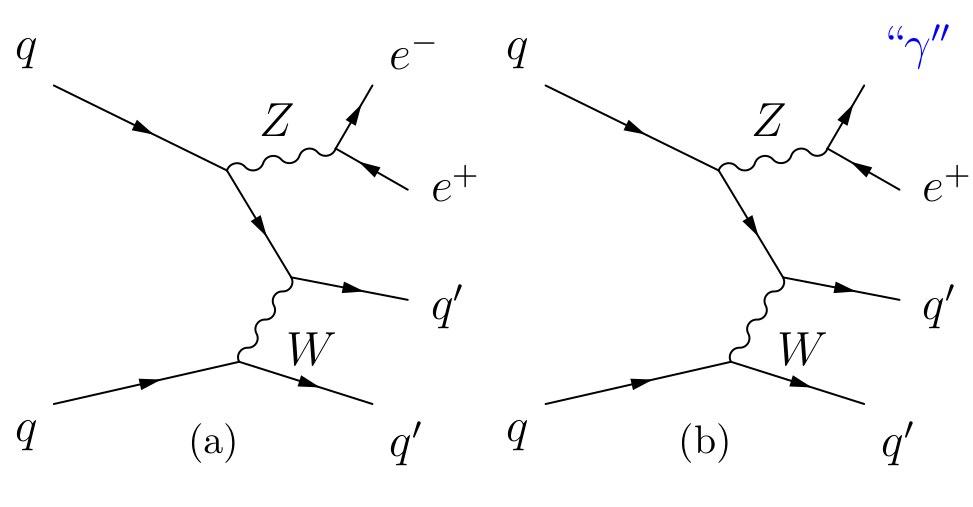
\includegraphics[width=.8\textwidth]{../../Thesis/ThesisImages/ZeeFakeDiagram.png}\\
\end{centering}
Want to be able to correct the number of fake photons predicted in MC to those present in Data
}


\frame{\frametitle{Fake Rate Object Selection}
\begin{itemize}
\item Want to calculate fake rate in events which could enter the signal region.
\item Create 2 control regions: $Z\rightarrow ee$ and $Z\rightarrow e \gamma$
\item Require:
	\begin{itemize}
	\item Common Object Selection (MET,Jets,Triggers, etc.)
	\item Exactly 1Bjet
	\item $Z\rightarrow ee:$ 2 Opposite Sign Electrons, 86.1 GeV $< m_{e^+ e^-} <$96.1 GeV
	\item $Z\rightarrow e\gamma :$1 Electron, $\geq$1 Photon,  86.1 GeV $< m_{e \gamma} <$96.1 GeV

	\end{itemize}
\item Tag and Probe Method used 
\item Systematic determined by varying tail size and other parameters
\end{itemize}
}

\frame{Data and MC \frametitle{$m_{ee}, m_{e\gamma}$}
\begin{columns}
\begin{column}{0.02\textwidth}
\rotatebox{90}{$m_{e\gamma}$ \qquad \qquad \qquad $m_{ee}$\qquad} 
%\rotatebox{90}{Muon Channel        } 
\end{column}
\begin{column}{0.48\textwidth}
\begin{itemize}
\item Data
\end{itemize}
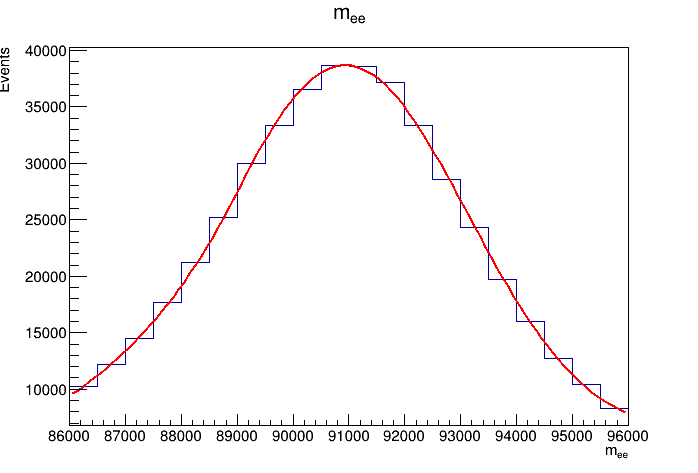
\includegraphics[width=.85\textwidth]{Images/Dataee.png} \\
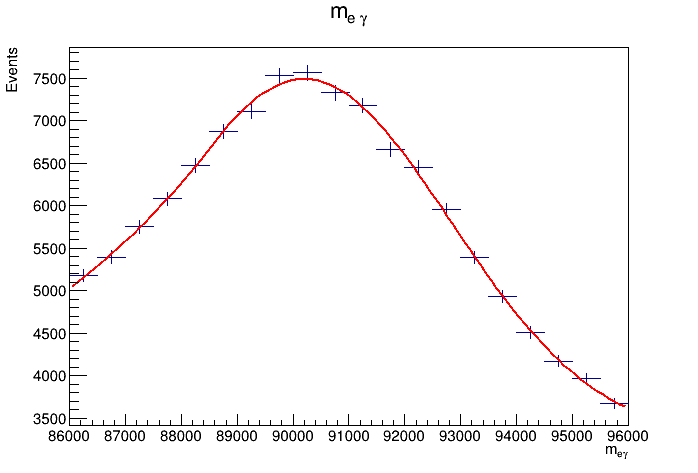
\includegraphics[width=.85\textwidth]{Images/Dataeg.png}
\end{column}
\begin{column}{0.48\textwidth}
\begin{itemize}
\item Monte Carlo
\end{itemize}
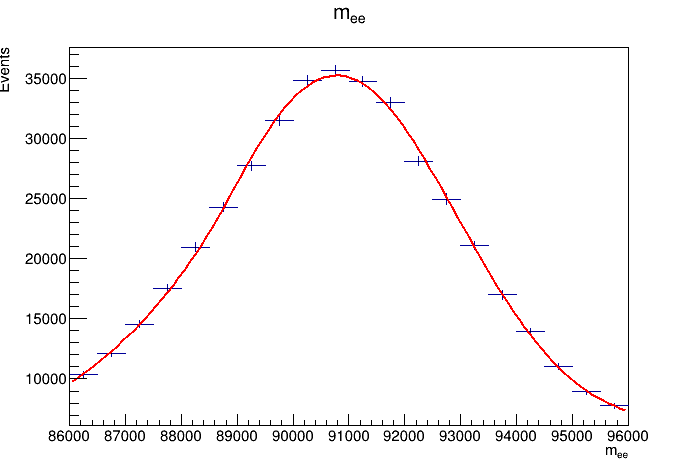
\includegraphics[width=.85\textwidth]{Images/MCVgamee.png} \\
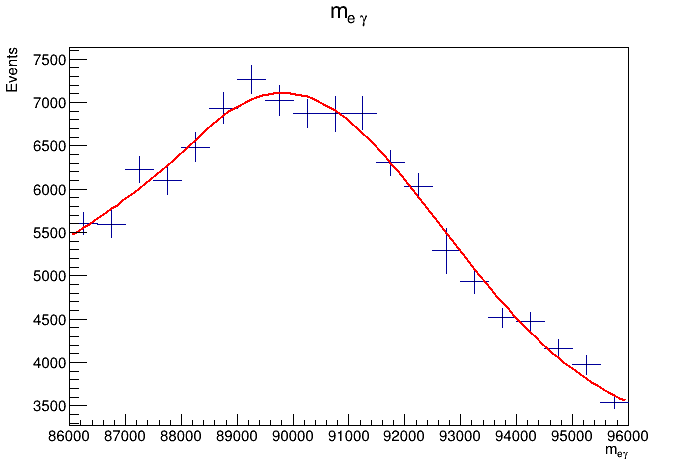
\includegraphics[width=.85\textwidth]{Images/MCVgameg.png}
\end{column}
\end{columns}
}


\frame{\frametitle{Scale Factor}
\[ \text{FR}^{\text{e-fake}}=\frac{N_{e,\gamma}}{N_{e,e}}\]

\[  \text{SF}^{\text{e-fake}}_{\text{FR}} = \frac{\text{FR}^{\text{e-fake}}_{\text{data}}}{\text{FR}^{\text{e-fake}}_{\text{MC}}}\]
Basic Scale Factor can be calculated for the entire spectrum:
$\text{SF}^{\text{e-fake}}_{\text{FR}} =0.97 \pm 0.01$\\
In practice this scale factor is calculated for converted and unconverted photons as well as in bins of $\eta$ and $\phi$
\begin{itemize}
\item Converted photons pair produce before the ECAL leaving tracks in the Inner Detector
\item Unconverted photons only pair produce inside of the ECAL
\end{itemize}
}

\frame{\frametitle{Data and MC Distributions}
\begin{columns}
\begin{column}{0.02\textwidth}
\rotatebox{90}{MC \qquad \qquad Data\qquad} 
%\rotatebox{90}{Muon Channel        } 
\end{column}
\begin{column}{0.32\textwidth}
\begin{itemize}
\item Probe $e$
\end{itemize}
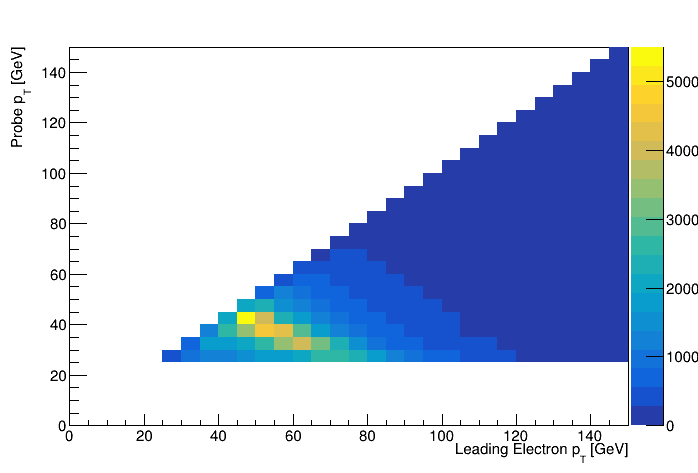
\includegraphics[width=.95\textwidth]{../../Thesis/ThesisImages/SearchStrategy/FakeRates/2dEEptDa.png} \\
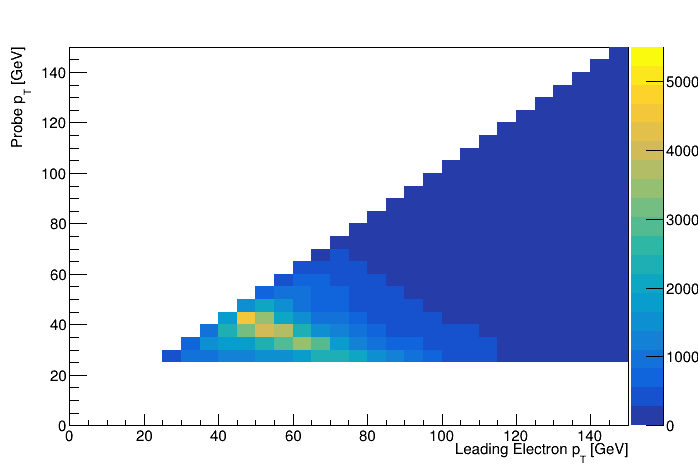
\includegraphics[width=.95\textwidth]{../../Thesis/ThesisImages/SearchStrategy/FakeRates/2dEEptMC.png} \\
\end{column}
\begin{column}{0.32\textwidth}
\begin{itemize}
\item Converted $\gamma$
\end{itemize}
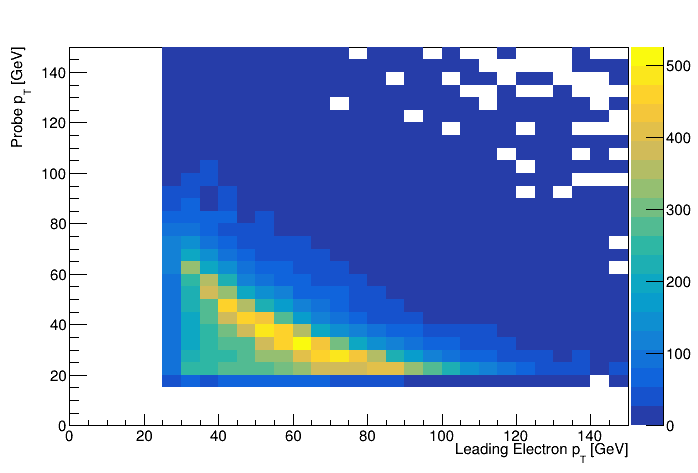
\includegraphics[width=.95\textwidth]{../../Thesis/ThesisImages/SearchStrategy/FakeRates/2dEPConvertedptDa.png} \\
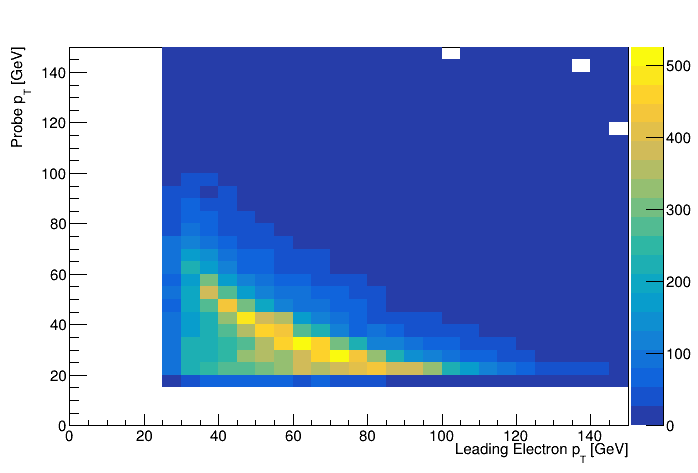
\includegraphics[width=.95\textwidth]{../../Thesis/ThesisImages/SearchStrategy/FakeRates/2dEPConvertedptMC.png}
\end{column}
\begin{column}{0.32\textwidth}
\begin{itemize}
\item Unconverted $\gamma$
\end{itemize}
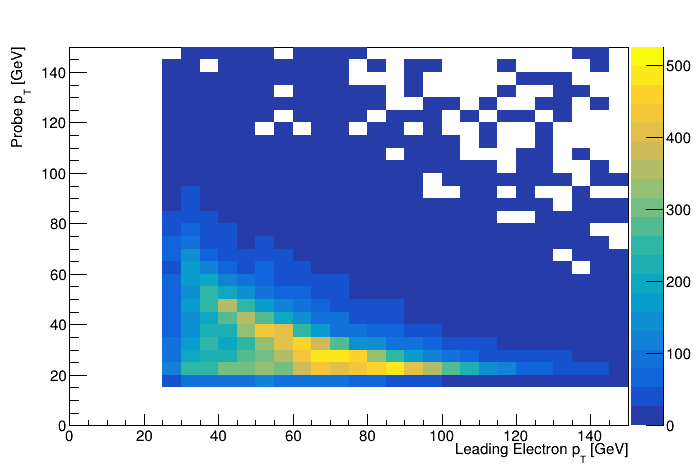
\includegraphics[width=.95\textwidth]{../../Thesis/ThesisImages/SearchStrategy/FakeRates/2dEPUnconvertedptDa.png} \\
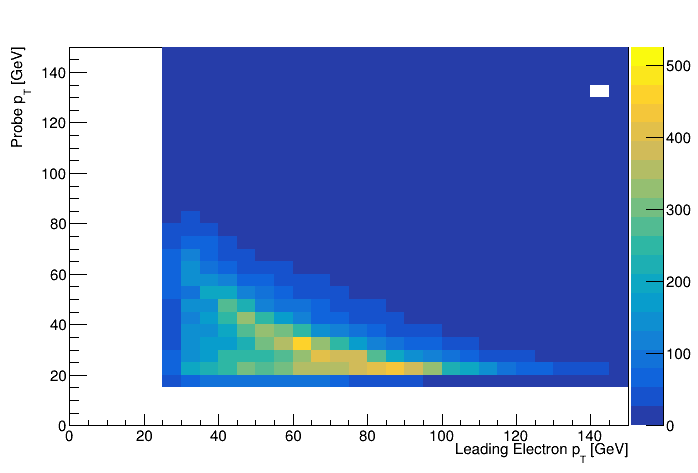
\includegraphics[width=.95\textwidth]{../../Thesis/ThesisImages/SearchStrategy/FakeRates/2dEPUnconvertedptMC.png}
\end{column}
\end{columns}
}

\frame{\frametitle{2D Fake Rates}
\begin{columns}
\begin{column}{0.48\textwidth}
\begin{itemize}
\item Converted $\gamma$
\end{itemize}
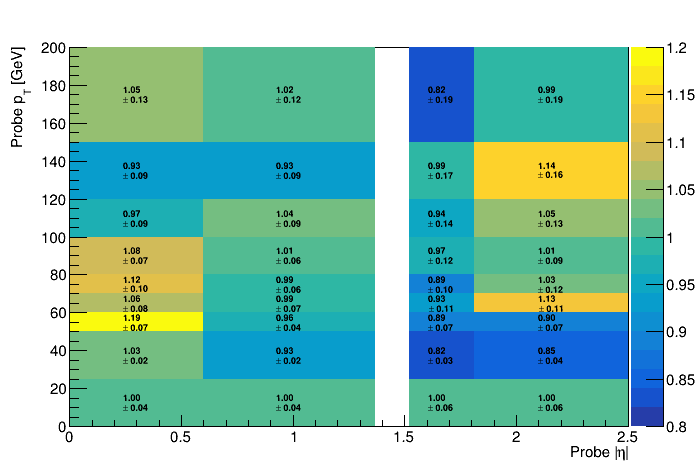
\includegraphics[width=.95\textwidth]{../../Thesis/ThesisImages/SearchStrategy/FakeRates/2DConverted.png}
\end{column}
\begin{column}{0.48\textwidth}
\begin{itemize}
\item Unconverted $\gamma$
\end{itemize}
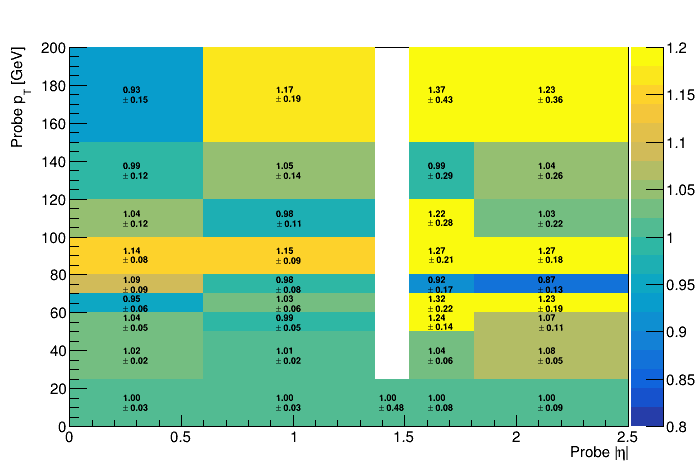
\includegraphics[width=.95\textwidth]{../../Thesis/ThesisImages/SearchStrategy/FakeRates/2DUnconverted.png}
\end{column}
\end{columns} 
}


\subsection{$j\rightarrow \gamma$ Fake Rate Studies: ABCD Method}

\frame{\frametitle{$j\rightarrow \gamma$ Fake Rate Studies}
Majority of hadronic fake photons from from $t\bar{t}$ events where a final state jet radiates a non-prompt photon.  Similarly  radiated photons for W+jets and single top processes can enter the signal region through the radiation of a non-prompt photon. \\
\begin{centering}
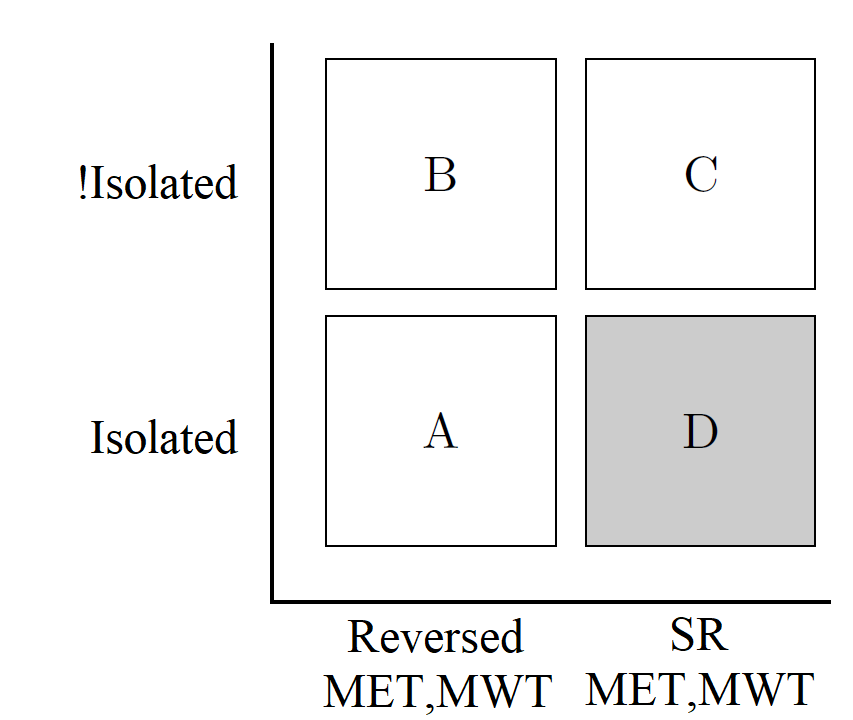
\includegraphics[width=.5\textwidth]{../../Thesis/ThesisImages/SearchStrategy/ABCDpictoral.png}\\
\end{centering}
}

\frame{\frametitle{ABCD Method}
\begin{columns}
\begin{column}{0.48\textwidth}
\[\frac{N_D^{\text{h-fake}}}{N_C^{\text{h-fake}}}=\frac{N_A^{\text{h-fake}}}{N_B^{\text{h-fake}}}
\text{ and }
\frac{N_D^{\text{h-fake}}}{N_A^{\text{h-fake}}}=\frac{N_C^{\text{h-fake}}}{N_B^{\text{h-fake}}}
\]
Want uncorrelated variables, use a correction factor to account to ensure closure\linespread{1.5}
\[\theta_{\text{MC}}=\frac
{\sfrac{N_\text{D,MC}^{\text{h-fake}}}{N_\text{C,MC}^{\text{h-fake}}}}
{\sfrac{N_\text{A,MC}^{\text{h-fake}}}{N_\text{B,MC}^{\text{h-fake}}}}\]
\[N_\text{D,est.}^{\text{h-fake}} = \frac{N_\text{A,data}^{\text{h-fake}}\times N_\text{C,data}^{\text{h-fake}}}{N_\text{B,data}^{\text{h-fake}}}\times \theta_\text{MC}
\]
\end{column}
\begin{column}{0.48\textwidth}
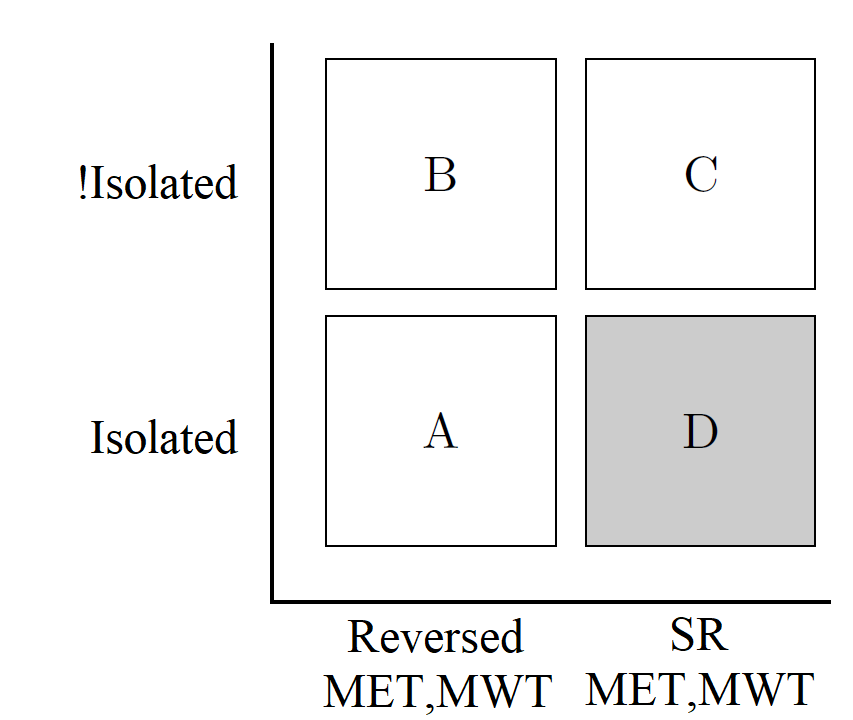
\includegraphics[width=.95\textwidth]{../../Thesis/ThesisImages/SearchStrategy/ABCDpictoral.png}
\[\text{SF}^\text{h-fake} = \frac{N^\text{h-fake}_\text{D,est.}}{N^\text{h-fake}_\text{D,MC}}
\]
\end{column}

\end{columns}
}

%
\frame{\frametitle{}

\begin{columns}
\begin{column}{0.02\textwidth}
\rotatebox{90}{$\mu$ channel  \qquad \qquad $e$ channel \qquad} 
%\rotatebox{90}{Muon Channel        } 
\end{column}
\begin{column}{0.48\textwidth}
\begin{itemize}
\item Converted Photons
%\item  MCee integral small range: 424,051.  - Vgam: 429789 - All 430225
%\item DATAee integral small range: 468,832
%\item MCeg integral small range: 110822     - Vgam: 115066 - All 152420
%\item DATAeg integral small range: 118198
\end{itemize}
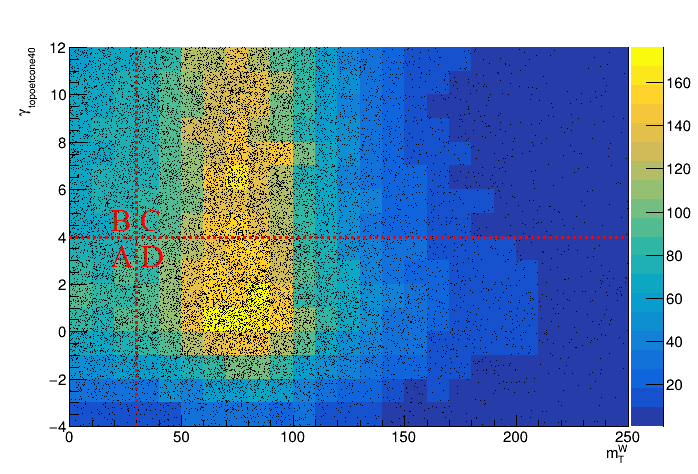
\includegraphics[width=.85\textwidth]{../../Thesis/ThesisImages/SearchStrategy/ABCD/ejetsConverted.png} \\
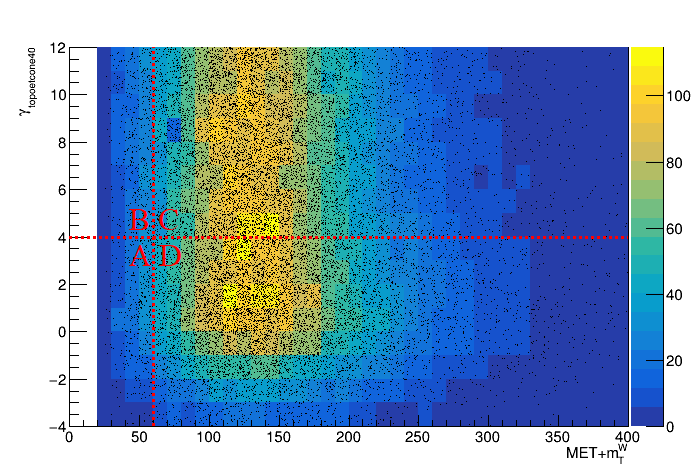
\includegraphics[width=.85\textwidth]{../../Thesis/ThesisImages/SearchStrategy/ABCD/mujetsConverted.png}
\end{column}
\begin{column}{0.48\textwidth}
\begin{itemize}
\item Unconverted Photons
\end{itemize}
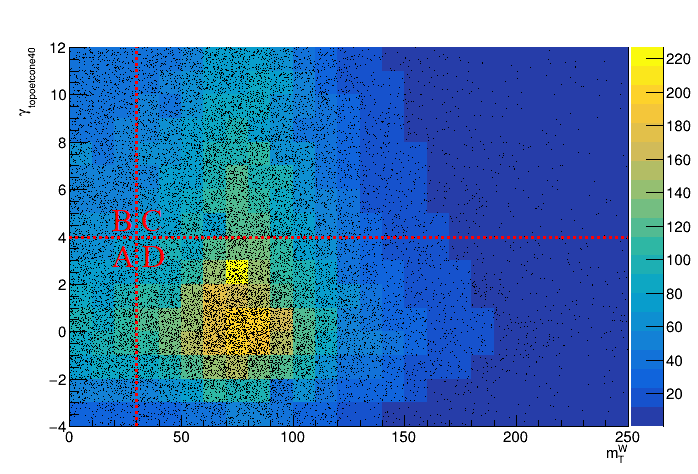
\includegraphics[width=.85\textwidth]{../../Thesis/ThesisImages/SearchStrategy/ABCD/ejetsUnconverted.png} \\
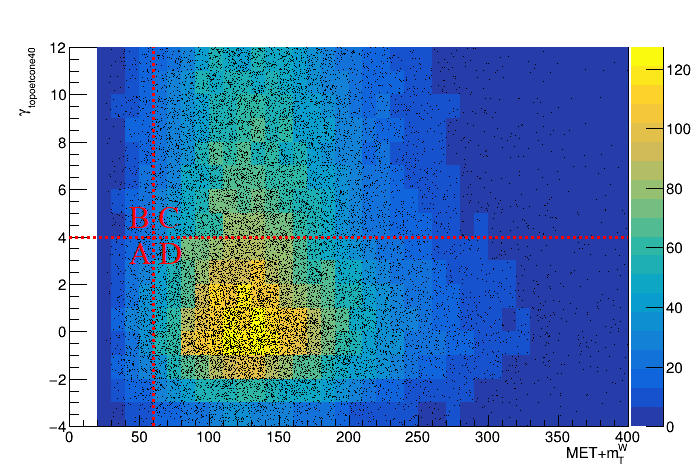
\includegraphics[width=.85\textwidth]{../../Thesis/ThesisImages/SearchStrategy/ABCD/mujetsUnconverted.png}
\end{column}
\end{columns}
\begin{table}[h]
\begin{center}
{\renewcommand{\arraystretch}{1.2}
\begin{tabular}{c|c|c}
\hline
Channel:     & Converted& Unconverted  \\  \hline 
Electron Channel  & $1.04\pm 0.14$     &   $2.27\pm 0.22$	\\ 
Muon Channel        & $1.64 \pm 1.40$   &   $2.27 \pm 0.41$\\ \hline %Change Put in post fit values
\end{tabular}
}
\end{center}
\end{table}
}

\section{Asimov Data Initial Fits}
\subsection{Asimov Fit, e+jets channel MC16a}
\frame{\frametitle{Asimov Data Fit}
\begin{columns}
\begin{column}{0.33\textwidth}
\begin{itemize}
\item VR1, W+$\gamma$
\end{itemize}
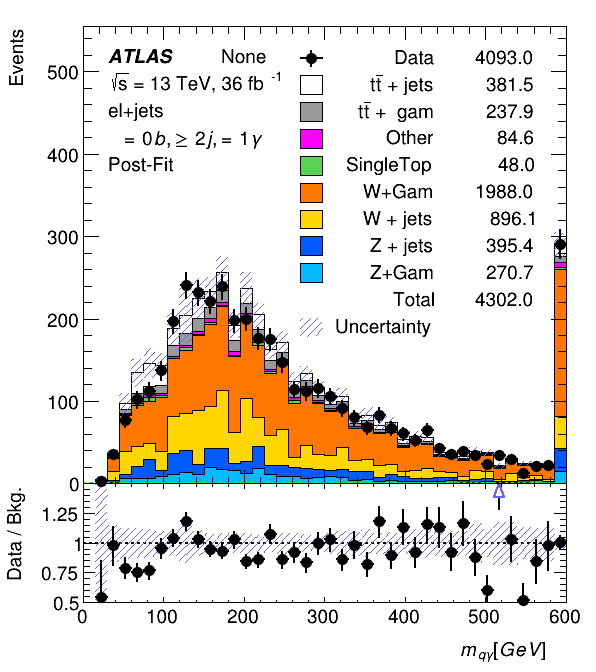
\includegraphics[width=.95\textwidth]{Images/FCNC_All_ejets/Plots/VR1_mqph_postFit.png} \\
\end{column}
\begin{column}{0.33\textwidth}
\begin{itemize}
\item VR2:  $t\bar{t}+\gamma$
\end{itemize}
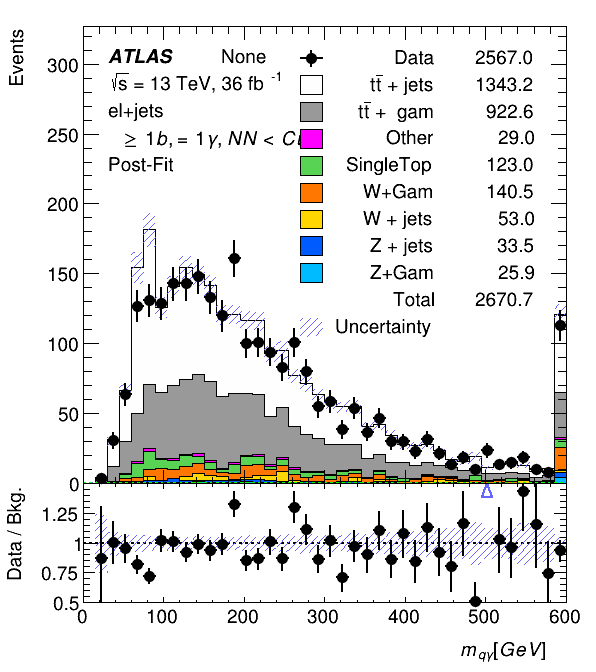
\includegraphics[width=.95\textwidth]{Images/FCNC_All_ejets/Plots/VR2_mqph_postFit.png} \\
\end{column}
\begin{column}{0.33\textwidth}
\begin{itemize}
\item Signal Region
\end{itemize}
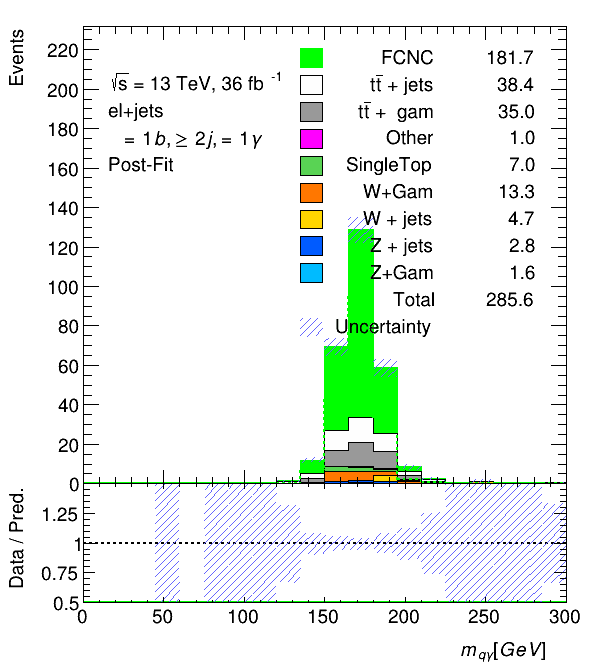
\includegraphics[width=.95\textwidth]{Images/FCNC_All_ejets/Plots/SR_mqph_postFit.png}
\end{column}

\end{columns}
Nominal signal strength $\mu = 1.0 \Rightarrow$ Branching Ratio = $10^{-3}$ \\
\hfill
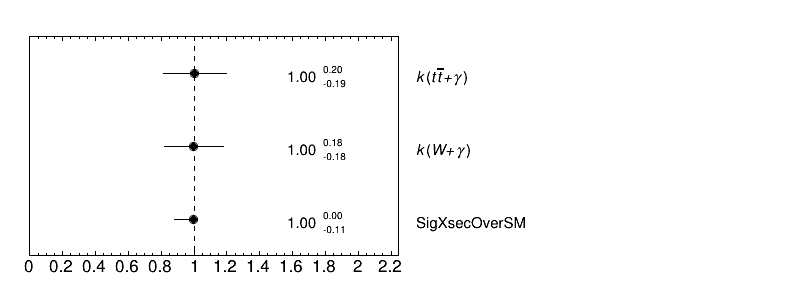
\includegraphics[width=.6\textwidth]{Images/FCNC_All_ejets/NormFactors.png}
\hfill
}

%\frame{\frametitle{Asimov Likelihood}
%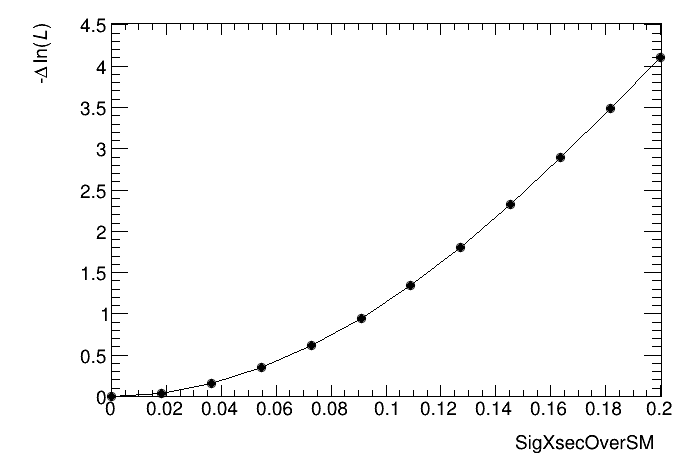
\includegraphics[width=.85\textwidth]{Images/FCNC_All_ejets/LHoodPlots/NLLscan_SigXsecOverSM.png} \\
%Wilk's Theorm allows us to use this as a goodness of fit technique.
%}

\frame{\frametitle{Statistical Limit from Asimov Fit}
\begin{itemize}
\item Expected signal strength $\mu= 0.13^{+0.05}_{-0.04}$
\item Corresponds to BR($t\rightarrow q \gamma$) = $13\times 10^{-5}$
\item Extrapolation to full data set limit: BR($t\rightarrow q \gamma$) $\approx 4\times 10^{-5}$
\end{itemize}
%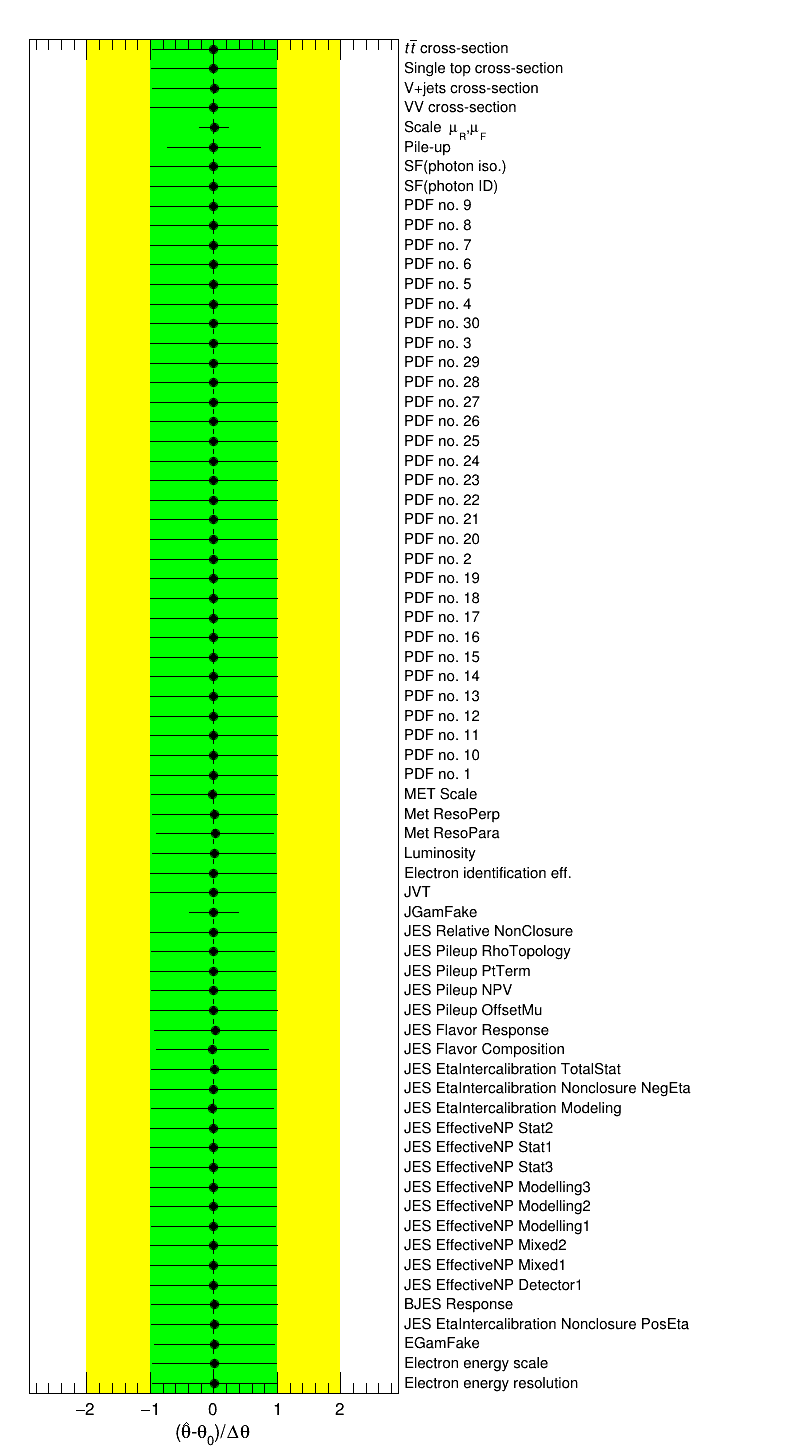
\includegraphics[width=.3\textwidth]{Images/FCNC_All_ejets/NuisPar.png}
%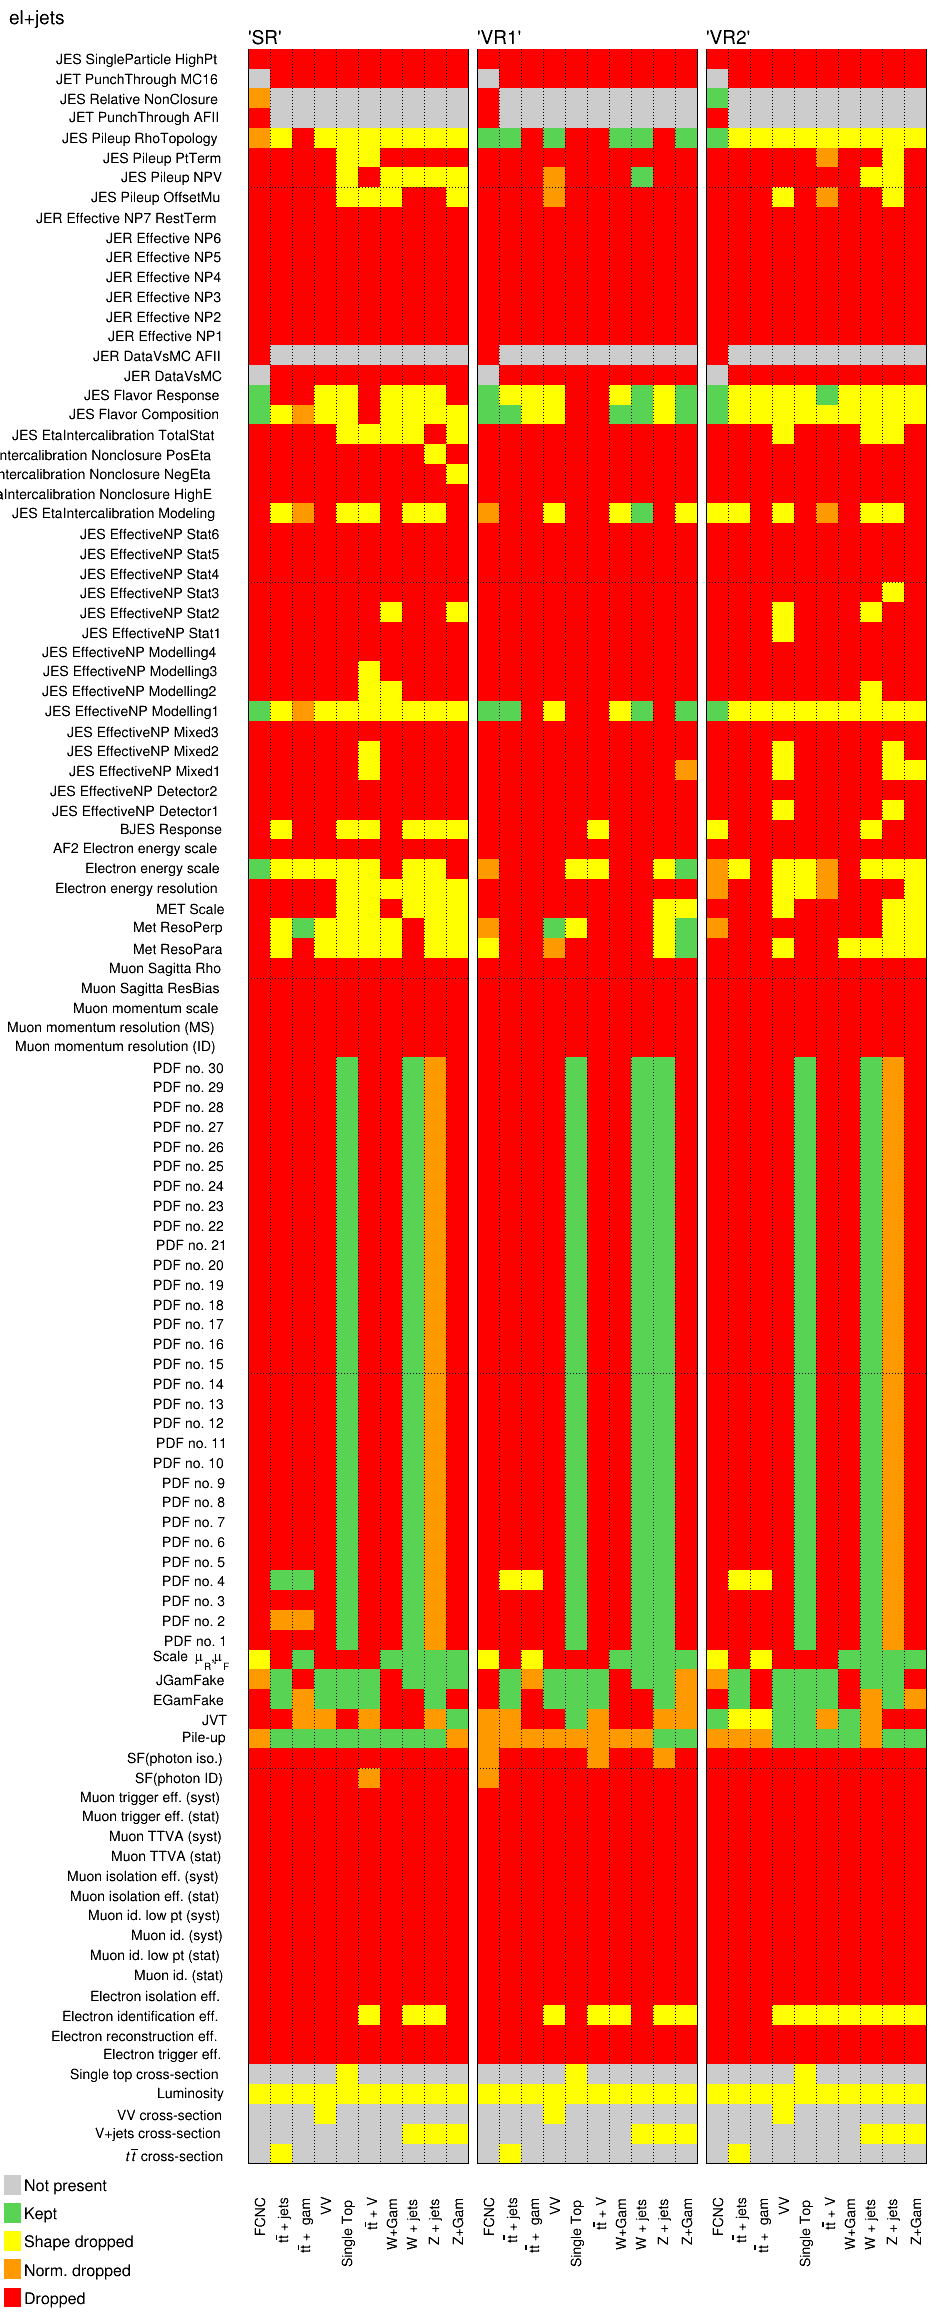
\includegraphics[width=.3\textwidth]{Images/FCNC_All_ejets/Pruning.png}
}
%%%%%%%%%%%%%%%%%%%%%%%%%%%%%%%%%%%%%%%%%%%%%%%%%%%%%%%%%%%%%%%%%%
\section{Outlook and Conclusions}

\frame{\frametitle{Outlook}
\begin{itemize}
\item Fake rates have been calculated and applied
\item Full systematics samples (slowly) running on the grid
\item Fitting machinery mostly in place now, should be ready once samples finish
\item Questions?
\end{itemize}
}



%%%%%%%%%%%%%%%%%%%%%%%%%%%%%%%%%%%%%%%%%%%%%%%%%%%%%%%%%%%%%%%%

\appendix
\section{Backup}
\frame{\frametitle{Backup}
}
\frame{\frametitle{FCNC Diagrams}
\centering
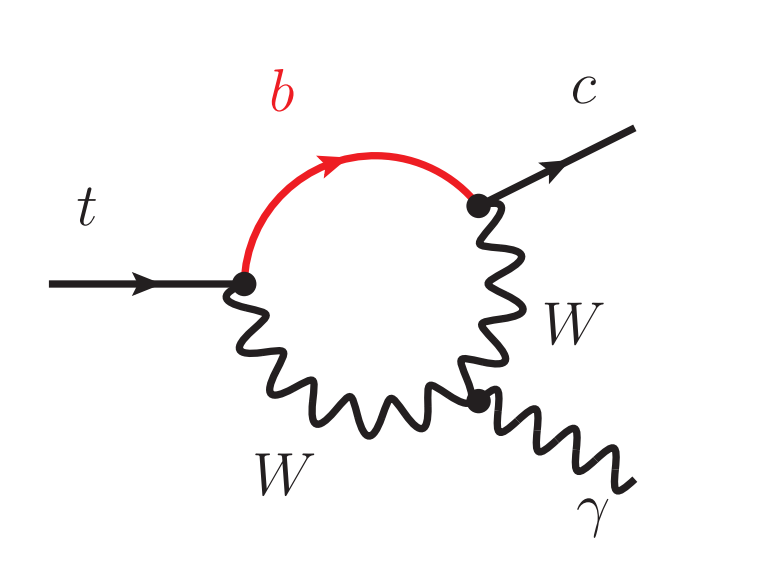
\includegraphics[width=.4\textwidth]{../../Thesis/ThesisImages/Theory/FCNCLoop.png}
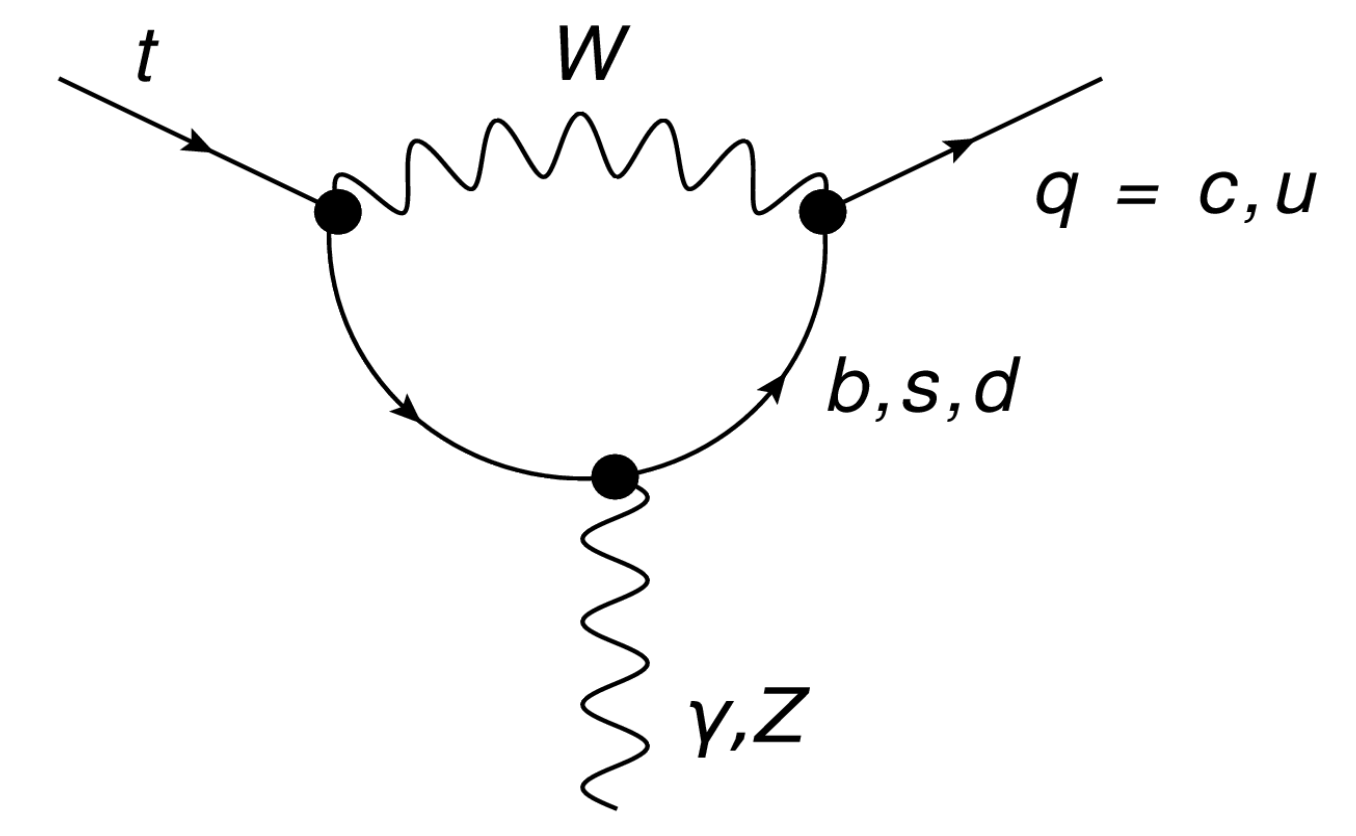
\includegraphics[width=.4\textwidth]{../../Thesis/ThesisImages/penguinFCNC.png}
}

\frame{\frametitle{No Photon Region SF Applied in Val Region}
\begin{columns}
\begin{column}{0.32\textwidth}
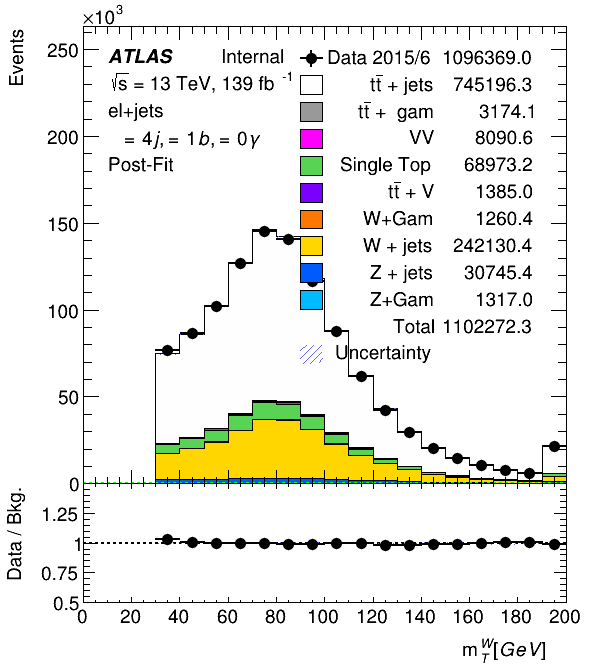
\includegraphics[width=.9\textwidth]{../../Thesis/ThesisImages/RegionPlots/AfterScaling/ControlRegions/HardCodedNormFactor/FCNC_All_ejets/Plots/VR3_MWT_postFit.png} \\
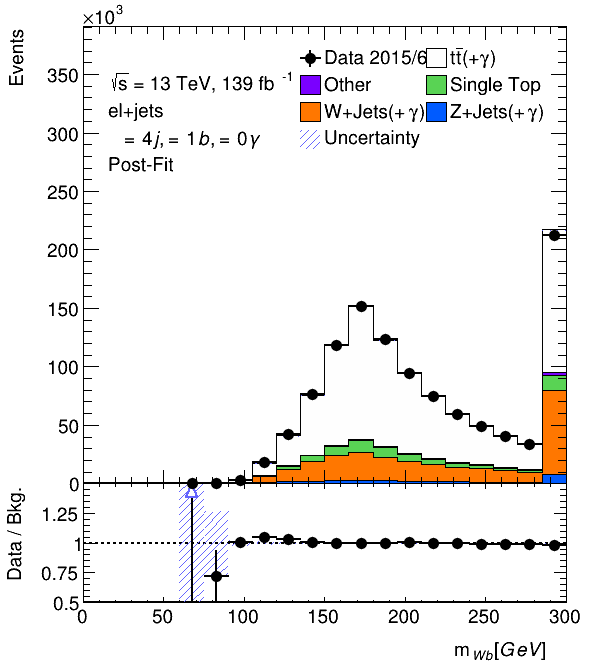
\includegraphics[width=.9\textwidth]{../../Thesis/ThesisImages/RegionPlots/AfterScaling/ControlRegions/HardCodedNormFactor/FCNC_All_ejets/Plots/VR3_SMtop_postFit.png} \\
\end{column}
\begin{column}{0.32\textwidth}
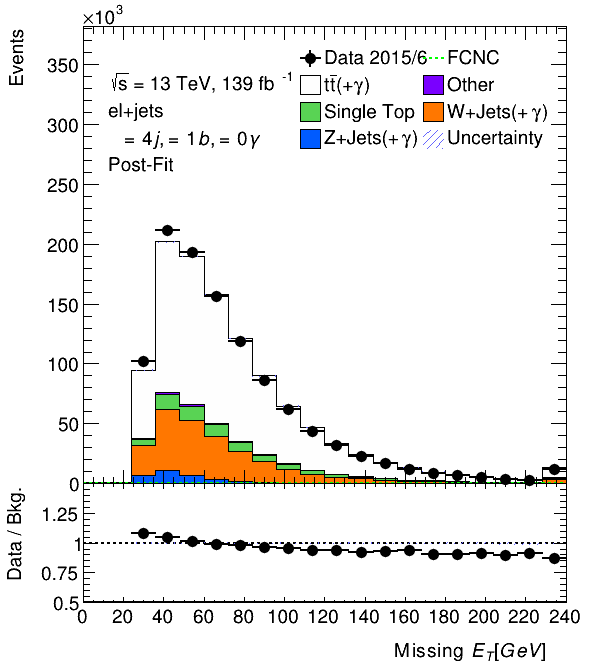
\includegraphics[width=.9\textwidth]{../../Thesis/ThesisImages/RegionPlots/AfterScaling/ControlRegions/HardCodedNormFactor/FCNC_All_ejets/Plots/VR3_met_postFit.png} \\
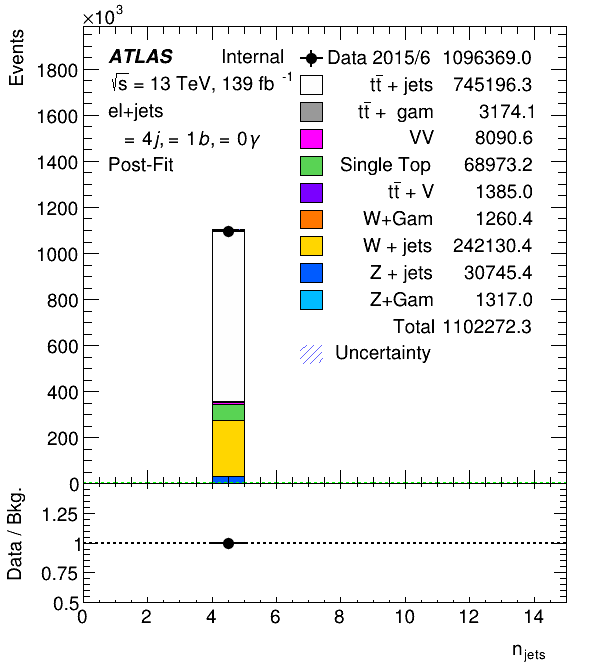
\includegraphics[width=.9\textwidth]{../../Thesis/ThesisImages/RegionPlots/AfterScaling/ControlRegions/HardCodedNormFactor/FCNC_All_ejets/Plots/VR3_njet_postFit.png}
\end{column}
\begin{column}{0.32\textwidth}
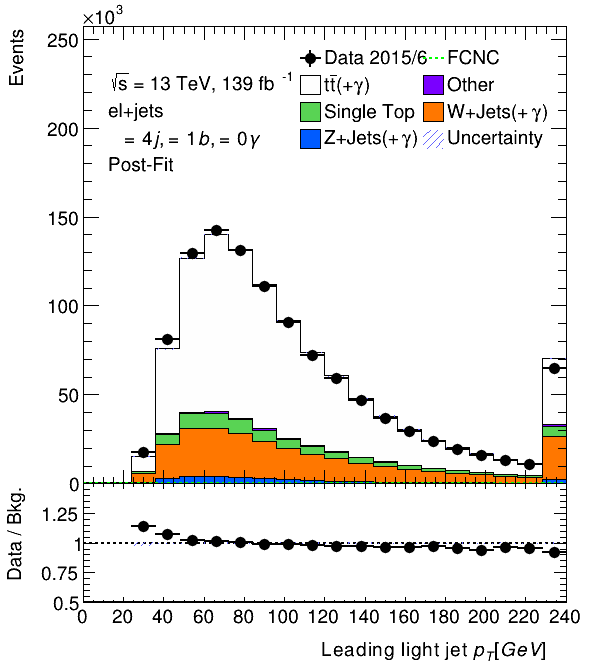
\includegraphics[width=.9\textwidth]{../../Thesis/ThesisImages/RegionPlots/AfterScaling/ControlRegions/HardCodedNormFactor/FCNC_All_ejets/Plots/VR3_jet0_pt_postFit.png} \\
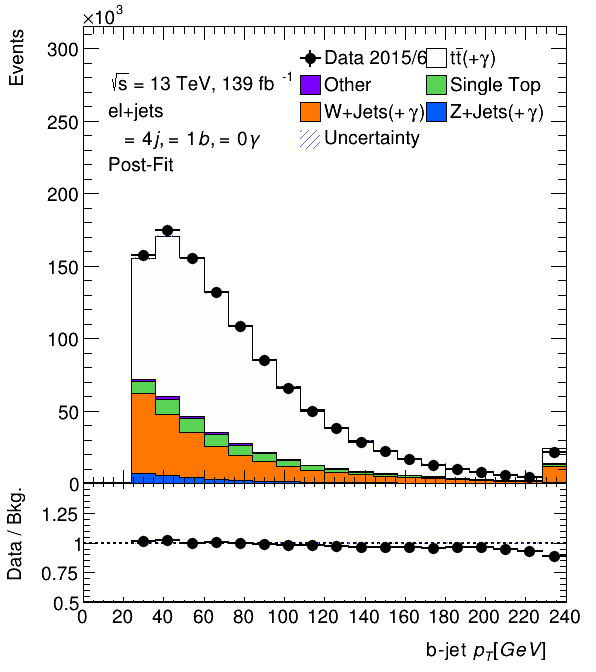
\includegraphics[width=.9\textwidth]{../../Thesis/ThesisImages/RegionPlots/AfterScaling/ControlRegions/HardCodedNormFactor/FCNC_All_ejets/Plots/VR3_bjet0_pt_postFit.png}
\end{column}
\end{columns}
}


%\frame{\frametitle{}
%}

%\frame{\frametitle{Neural Network Model Inputs}
%\centering
%\scalebox{0.8}{ $\text{Separation} = \sum_{i}^{bins} \frac {n_{s i}-n_{b i}}{n_{s i}+n_{b i}}$}
%\begin{columns}
%\begin{column}{0.48\textwidth}
%\centering
%mu+jets channel\\
%\scalebox{0.6}{\begin{tabular}{cc}
%Variable & Separation \\
%\hline
%photon0iso & 41.18 \\
%mqgam & 28.27 \\
%photon0pt & 24.07 \\
%mtSM & 11.60 \\
%mlgam & 7.56 \\
%deltaRjgam & 5.64 \\
%deltaRbl & 4.42 \\
%MWT & 3.34 \\
%ST & 3.30 \\
%nuchi2 & 3.12 \\
%jet0pt & 2.81 \\
%njets & 2.07 \\
%smchi2 & 1.89 \\
%wchi2 & 1.87 \\
%jet0e & 1.52 \\
%deltaRlgam & 1.17 \\
%leptone & 0.87 \\
%deltaRjb & 0.86 \\
%met & 0.68 \\
%bjet0pt & 0.52 \\
%leptoniso & 0.27 \\
%\end{tabular}
%}
%\end{column}
%\begin{column}{0.48\textwidth}
%\centering
%e+jets channel \\
%\scalebox{0.6}{\begin{tabular}{c c}
%Variable & Separation\\
%\hline
%photon0pt & 23.14 \\
%mqgam & 22.73 \\
%photon0iso & 18.70 \\
%mtSM & 11.02 \\
%mlgam & 9.53 \\
%deltaRbl & 5.00 \\
%deltaRjgam & 4.60 \\
%ST & 3.83 \\
%MWT & 3.16 \\
%jet0pt & 2.47 \\
%njets & 1.70 \\
%nuchi2 & 1.59 \\
%deltaRlgam & 1.40 \\
%wchi2 & 1.33 \\
%smchi2 & 1.09 \\
%deltaRjb & 0.88 \\
%leptone & 0.85 \\
%leptoniso & 0.56 \\
%bjet0pt & 0.50 \\
%met & 0.47 \\
%\end{tabular}
%}
%\end{column}
%\end{columns}
%}
%
%	\frame{\frametitle{Input Variables}
%	['photon0iso','photon0pt','mqgam','mlgam','mtSM','deltaRjgam','deltaRbl',\\
%	'MWT','ST','njets','wchi2','jet0pt','deltaRlgam','leptone','met','bjet0pt']
%	
%	
%	}

%\frame{\frametitle{Integrated Luminosity}
%\centering
%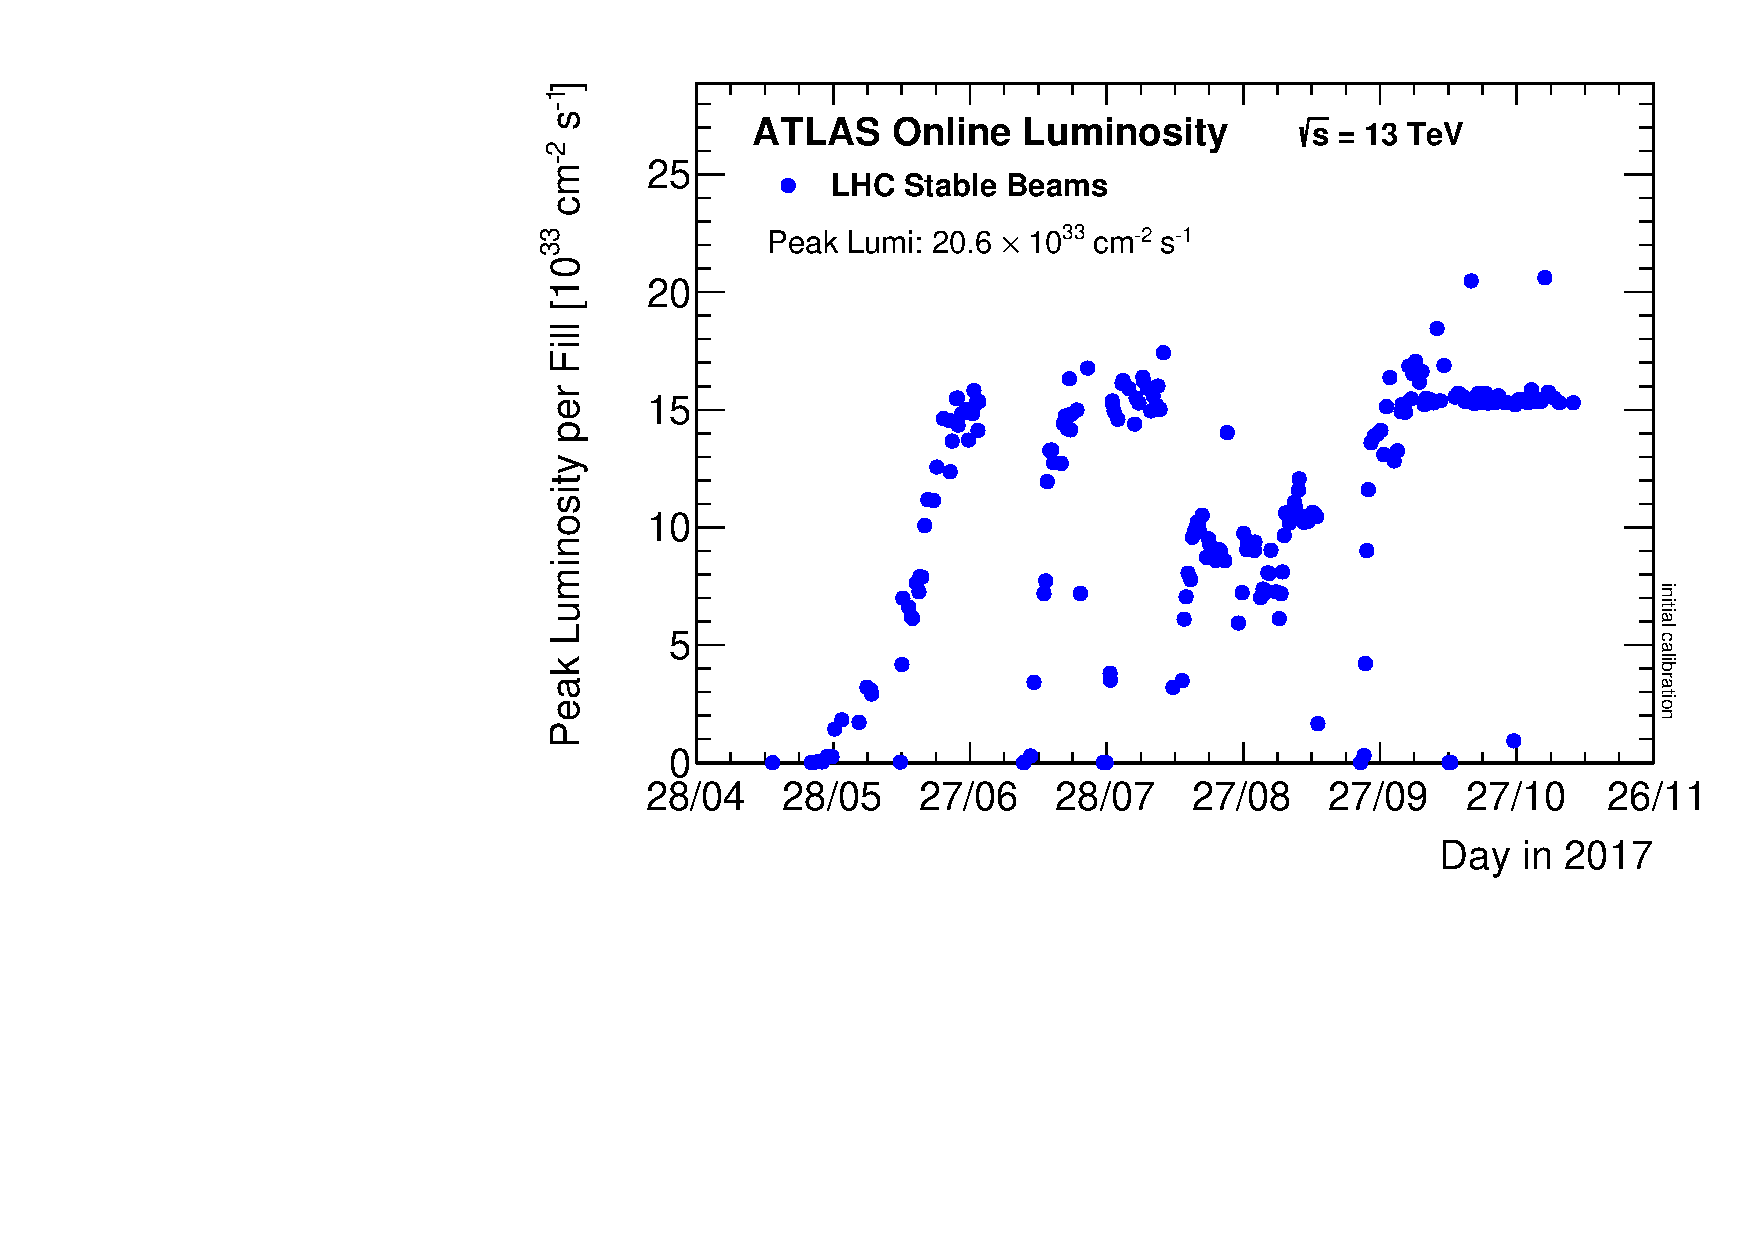
\includegraphics[width=1.\textwidth]{../../Thesis/ThesisImages/2017PeakLumiByFill.pdf}
%}
%\frame{\frametitle{A Couple BSM Diagrams}
%\centering
%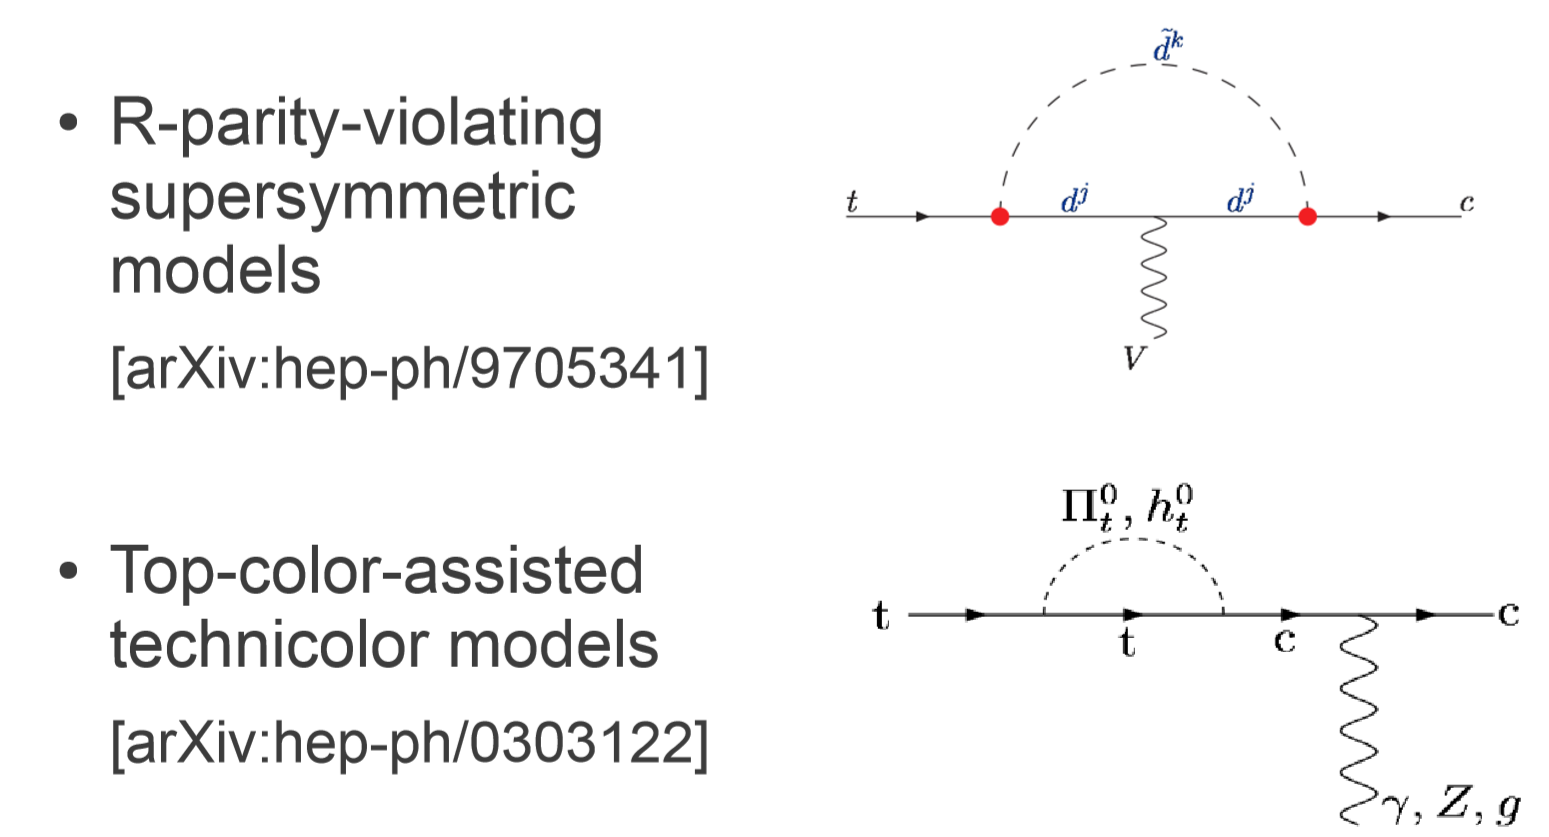
\includegraphics[width=1.\textwidth]{../../Thesis/ThesisImages/BSMDiagrams.png}
%}

\frame{\frametitle{Jets/AntiKT}

\[ d_{ij} = min(\frac{1}{p_{ti}^2},\frac{1}{p_{tj}^2}) \frac{\Delta_{ij}^2}{R^2}
\]
\[ d_{iB} = \frac{1}{p_{ti}^2}
\]
\[ \Delta_{ij}^2 = (\eta_i -\eta_j )^2 + (\phi_i - \phi_j )^2
\]
\begin{itemize}
\item Find minimum of entire set of $\{ d_{ij},d_{iB} \}$
\item If $d_{ij}$ is the minimum particles i,j are combined into one particle and removed from the list of particles
\item If $d_{iB}$ is the minimum i is labelled as a final jet and removed from the list of particles
\item Repeat until all particles are part of a jet with distance between jet axes $\Delta_{ij}$ is greater than R
\end{itemize}
}

%\frame{\frametitle{B-tagging}
%\centering
%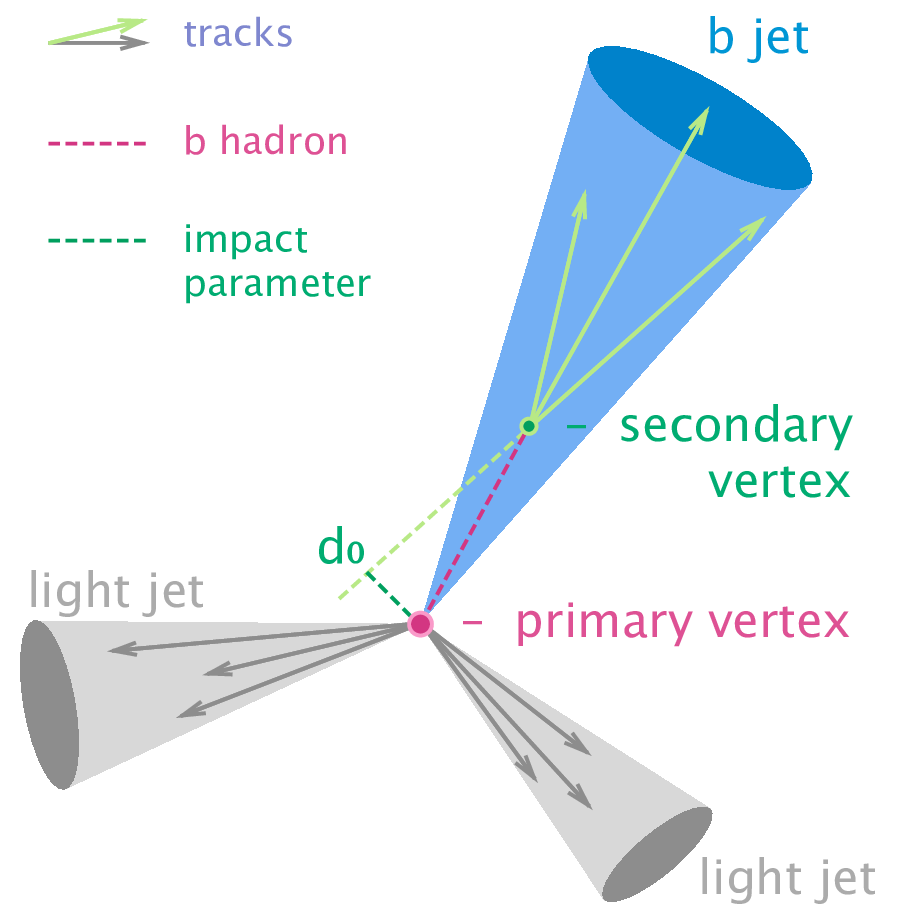
\includegraphics[height=.8\textheight]{../../Thesis/ThesisImages/SimulationNN/B-tagging_diagram.png}
%}

\frame{\frametitle{}
\[ \mathcal{L}^{eff}_{tq\gamma} = - e \bar{c} \frac{i \sigma^{\mu\nu}q_{\nu}}{m_t}(\lambda^{L}_{ct}P_L + \lambda^{R}_{ct}P_{R}) t A_{\mu} +H.c.
\]
}

\end{document}

%36.070


%%% Neural Net Ref: http://cs231n.github.io/neural-networks-1/

% npart0=['photon0_iso','photon0_pt','m_qgam','m_lgam','m_tSM','deltaRjgam','deltaRbl','MWT','S_T','nbjets','njets','w_chi2','jet0_pt','nu_chi2','sm_chi2','deltaRlgam','lepton_e','met','lepton_iso','bjet0_pt']
%all vars

%npart = ['photon0_iso','photon0_pt','m_qgam','m_lgam','m_tSM','deltaRjgam','deltaRbl','MWT','S_T','njets','nbjets','w_chi2','jet0_pt','deltaRlgam','lepton_e','met','bjet0_pt']
%usual npart1

%npart1=['photon0_iso','photon0_pt','deltaRjgam','deltaRbl','MWT','S_T','njets','w_chi2','jet0_pt','deltaRlgam','lepton_e','met','bjet0_pt']
%minimal